%%% AAMAS 2027 main-track draft (GAAI). Anonymous review.
%%% Official AAMAS 2027 class (aamas.cls).
%%% Compile: pdflatex main && bibtex main && pdflatex main && pdflatex main
\PassOptionsToPackage{expansion=false}{microtype}
\documentclass[sigconf,anonymous]{aamas}
\microtypesetup{expansion=false,protrusion=false}

\usepackage{balance}
\usepackage{booktabs}
\usepackage{tikz}
\usetikzlibrary{arrows.meta,positioning,fit,calc}
\usepackage{enumitem}

\newcommand{\task}[1]{\texttt{#1}}
\newcommand{\A}{\mathcal{A}}
\newcommand{\Acap}{\mathcal{A}^{\cap}}
\newcommand{\STS}{\mathrm{STS}}

%%% AAMAS-2027 copyright block (do not change!)
\makeatletter
\gdef\@copyrightpermission{
  \begin{minipage}{0.2\columnwidth}
   \href{https://creativecommons.org/licenses/by/4.0/}{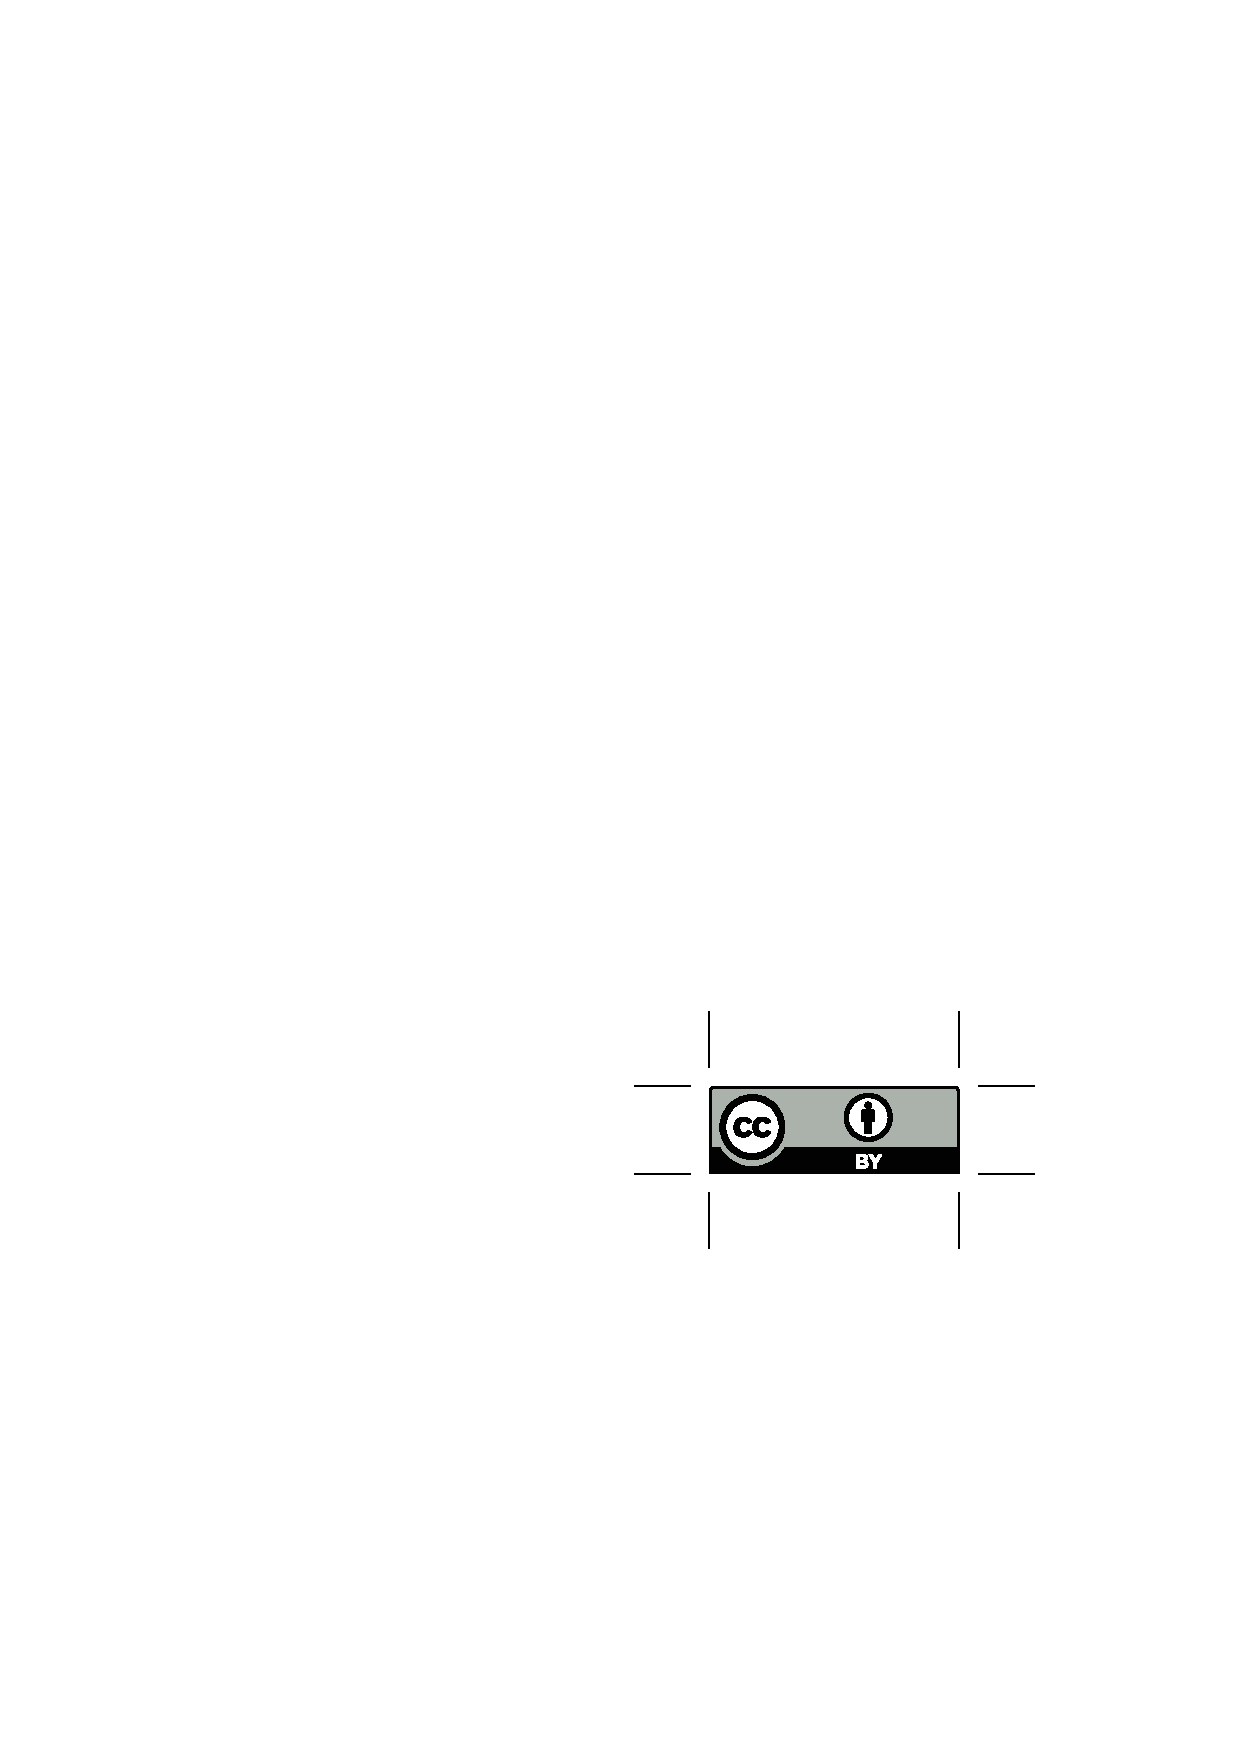
\includegraphics[width=0.90\textwidth]{by}}
  \end{minipage}\hfill
  \begin{minipage}{0.8\columnwidth}
   \href{https://creativecommons.org/licenses/by/4.0/}{This work is licensed under a Creative Commons Attribution International 4.0 License.}
  \end{minipage}
  \vspace{5pt}
}
\makeatother

\setcopyright{ifaamas}
\acmConference[AAMAS 2027]{Proc.\@ of the 26th International Conference on Autonomous Agents and Multiagent Systems (AAMAS 2027)}{3--7 May 2027}{Hanoi, Vietnam}{M.~Baldoni, F.~Fang, W.~Yeoh, N.~Yorke-Smith (eds.)}
\copyrightyear{2027}
\acmYear{2027}
\acmDOI{}
\acmISBN{}
\acmSubmissionID{TODO-FILL-OPENREVIEW-ID}
\submissionType{Research Paper Track}

\title{What Does a Computer-Use Agent Reliability Score Actually Measure?}

\begin{document}
\begin{abstract}
A computer-use agent (CUA) reliability score is treated as if it observed whether the agent did the task.
It does not.
The score is a constructed measurement: a pipeline that turns a trajectory into candidate evidence, a decision, a reported value, and eventually a selection.
We audit one frozen instrument on MyPCBench with three studies that share an instrument family rather than three independent experiments; no study's sample is pooled with another's.
The \emph{core} result opens the evaluator at the candidate-evidence stage.
On a sealed 134-trajectory, 61-task corpus, the frozen extractor misses 39 of 59 observations for which recoverable evidence existed; on 13 of those 39 misses, gold was already in the extractor's own accumulated candidate set and a fail-closed aggregation rule discarded it (M1a; majority-gold in 7/13).
A locked repair of exactly those 13 cases (R-AGG) moves a downstream ranking statistic $+8$ correct $/-18$ wrong; treating every extractor hit as gold (ALL) is worse, not better ($+10/-20$).
No tested repair dominates, and a channel-layer intervention inverts an ordering statistic on the one common-support cluster where it is defined ($n_{\mathrm{eff}}=1$), by destroying one lane's evidence while leaving the other unchanged.
A locked, corpus-independent reconstruction rule recovers 9 of 30 hand-written label components.
Two \emph{supporting} checks, on the same family and protocol, show why this audit is necessary rather than optional: the reported score can stay put or move without a corresponding change in what the agent actually tracked (Study~1, 24 valid pairs), and a pre-registered confirmatory selection test cannot be evaluated because coverage --- not the score --- gates which agents are even eligible to be ranked (Study~2: 9, 8, and 1 valid pairs out of 57 legs each; $n_{\min}=3$ excludes one of three agents).
A CUA leaderboard number is downstream of correspondence, not a substitute for it.
\end{abstract}

\begin{CCSXML}
<ccs2012>
<concept>
<concept_id>10010147.10010178.10010199</concept_id>
<concept_desc>Computing methodologies~Intelligent agents</concept_desc>
<concept_significance>500</concept_significance>
</concept>
<concept>
<concept_id>10002944.10011122.10002945</concept_id>
<concept_desc>General and reference~Evaluation</concept_desc>
<concept_significance>500</concept_significance>
</concept>
</ccs2012>
\end{CCSXML}
\ccsdesc[500]{Computing methodologies~Intelligent agents}
\ccsdesc[500]{General and reference~Evaluation}

\keywords{computer-use agents, reliability, evaluation, measurement validity}

\maketitle

\section{Introduction}
\label{sec:intro}

Leaderboards for computer-use agents (CUAs) report a completion-conditioned score: the episode ended, and a rubric assigned a number~\citep{jang2026mypcbench,xie2024osworld,zhou2024webarena}.
That number is then used as if it were an observation of reliability --- to pick an agent, to claim progress, to close a run.
It is not an observation.
A score is a \emph{constructed measurement}~\citep{cronbach1955construct,messick1995validity,kane2013validating}: a chain of transformations from trajectory to candidate evidence to decision to reported value to selection.
Validity is a property of that chain, not of the scalar it emits.

Recent work has already shown that CUA scores can be wrong for reasons adjacent to this chain.
Dong et al.~\citep{dong2026misscore} document systematic misscoring of computer-use agents.
Xue et al.~\citep{xue2025illusion} show that web-agent ``progress'' can be an artifact of the evaluation setup rather than the agent.
Rosset et al.~\citep{rosset2026verifiers} treat verifier construction as the object of study, not a solved backend.
Those papers establish that scores can lie.
None of them locates the lie inside a frozen extractor's own candidate-evidence set, and none measures what a locked correspondence repair does to a published ranking statistic.
That is the gap this paper fills --- on one instrument, not as a survey of judges.

\paragraph{Core.}
The empirical core is a correspondence audit of a frozen extractor at the candidate-evidence stage (Study~3, \S\ref{sec:s3}).
On a sealed 134-trajectory corpus we ask whether gold was already in the extractor's accumulated candidate set when the decision failed to award it (criterion M1a).
It was, on 13 of 39 recall misses; gold was a strict majority of the accumulated candidates in 7 of those 13.
A locked repair of exactly those 13 cases moves a downstream ranking statistic $+8/-18$; a looser repair that trusts every candidate is worse, not better ($+10/-20$).
No repair among six tested configurations dominates, and a channel-layer intervention inverts a comparative ordering statistic on the one task cluster where the frozen instrument defines it --- by destroying one lane's evidence, not by improving the other.
A locked, corpus-independent reconstruction rule recovers 9 of 30 hand-written label components.
The score is therefore not merely noisy: it is downstream of a correspondence step the leaderboard never reports, and rewriting that step --- even conservatively --- reorders the ranking.

\paragraph{Supporting.}
Two checks on the same family and protocol show why this audit is required rather than optional, not two more leaderboards.
Study~1 (\S\ref{sec:s1}) shows the score can remain invariant, or can move, without a corresponding change in what the agent actually tracked in the world.
Study~2 (\S\ref{sec:s2}) shows a pre-registered confirmatory selection test cannot be evaluated, because coverage --- not the score --- gates which agents are even eligible to be ranked.
Neither is a ranking result; together they motivate reading Study~3 as a measurement claim about the instrument, not a third leaderboard about the agents.

\paragraph{Contributions.}
\begin{enumerate}[leftmargin=*,itemsep=2pt,topsep=4pt]
\item \textbf{Core.} On a frozen CUA instrument, gold is already in the extractor's accumulated candidate set on 13/39 recall misses (M1a). No tested layer repair dominates; a channel-layer repair inverts a comparative ordering statistic by destruction, not improvement ($n_{\mathrm{eff}}=1$); a locked reconstruction rule recovers 9/30 hand-written label components. Correspondence, not coverage of the extractor, is the object.
\item \textbf{Supporting.} The score can dissociate from world tracking (Study~1, 24 valid pairs). A pre-registered confirmatory selection test is not evaluated because coverage, not score, determines the roster (Study~2, $n_{\min}=3$).
\item \textbf{Method.} One frozen pipeline, paired counterfactuals, a fail-closed termination channel disjoint from the judge, no pooling of $n$ across studies, no recommended repair.
\end{enumerate}

\paragraph{What this paper does not claim.}
It does not claim that computer-use agents are unreliable, that a repair should be shipped, or that rankings are unstable in general.
It does not rank models.
It does not transport M1a to OSWorld, WebArena, or any unfrozen judge.
A pre-specified comparative-scale gate required 20 independent task clusters; 16 of 28 candidates survived a frozen feasibility probe, so that experiment was not opened.
It reports what one frozen reliability score actually measures.

\section{A Frozen Measurement Pipeline}
\label{sec:pipeline}

\begin{figure}[t]
\centering
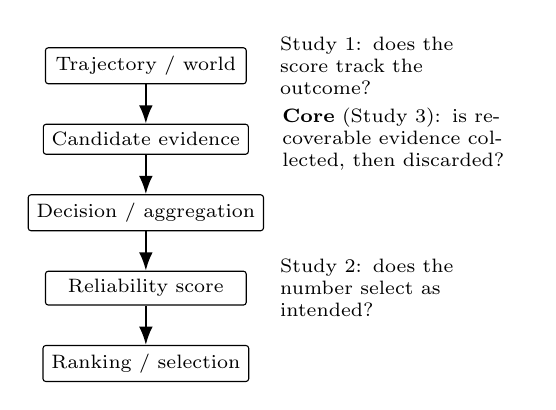
\begin{tikzpicture}[
  font=\scriptsize,
  box/.style={draw, rounded corners=1pt, align=center, inner sep=3pt, minimum width=2.55cm},
  arr/.style={-{Latex}, thick},
  note/.style={font=\scriptsize, align=left, text width=2.35cm}
]
\node[box] (traj) {Trajectory / world};
\node[box, below=5mm of traj] (ev) {Candidate evidence};
\node[box, below=5mm of ev] (dec) {Decision / aggregation};
\node[box, below=5mm of dec] (sc) {Reliability score};
\node[box, below=5mm of sc] (rk) {Ranking / selection};
\draw[arr] (traj) -- (ev);
\draw[arr] (ev) -- (dec);
\draw[arr] (dec) -- (sc);
\draw[arr] (sc) -- (rk);
\node[note, right=3mm of traj] {Study~1: does the score track the outcome?};
\node[note, right=3mm of ev, text width=3.0cm] {\textbf{Core} (Study~3): is recoverable evidence collected, then discarded?};
\node[note, right=3mm of sc] {Study~2: does the number select as intended?};
\end{tikzpicture}
\caption{The score is constructed. The core study opens the candidate-evidence and decision stages; the two supporting studies show why that audit is necessary rather than optional. No stage's count is pooled with another's.}
\Description{Four stacked boxes from trajectory to candidate evidence to decision/score to ranking, with Study 1, the core Study 3, and Study 2 annotated at different stages.}
\label{fig:pipeline}
\end{figure}

A CUA episode produces a trajectory $\tau$ in a guest world $E$, on MyPCBench~\citep{jang2026mypcbench}: a seeded virtual desktop.
For task $t$, $E_t^{0}$ is the seeded guest and $E_t^{1}=I_t(E_t^{0})$ applies a locked patch to a pre-registered determining set $D_t$.
Instruction, interface, screenshot size, and judge stay fixed; guest probes confirm that gold moved.
A pair is \emph{valid} only if both legs terminate under a fail-closed classifier that does not consult the judge: termination and score are disjoint channels.
Execution failure is an absent observation, not a tracking miss.

A reliability instrument $J$ does not observe reliability; it applies a sequence of maps: trajectory to candidate evidence, to a decision, to a reported score $S(\tau)$, to a selection.
Correspondence can fail at any map (Figure~\ref{fig:pipeline}).
Study~3 (core) inspects the candidate-evidence and decision maps directly.
Study~1 tests the composite $S(\tau)$ against the world.
Study~2 tests $S$ as a selection instrument against a tracking construct that never consults $J$.
Labels, windows, aggregation, and comparison rules for the extractor are held at a recorded commit throughout; repairs are diagnostic interventions on one layer at a time, not a proposed replacement metric.

\section{Core: Candidate Evidence Decides the Score}
\label{sec:s3}

\paragraph{Question.}
When the instrument fails to award gold, was gold already collected --- and if so, at what rate, and does fixing that one step change the reported ranking?

\paragraph{Corpus and lock.}
$N=134$ rows (one component of $D$ on one leg), 57 legs, 61 tasks, frozen extractor \texttt{3242c30}.
A row is \emph{R1-positive} if the gold value is literally present in the agent's answer ($n=59$: 20 MATCH + 39 RECALL\_MISS); the remaining 61 rows are ABSENT (gold is not in the text at all).
All rates below are conditional on these audited sets; they are not a false-negative rate of the agent or of the benchmark.
The corpus is sealed and $R$ is not revised after seeing outcomes.
Groundedness (G1) is 30/30 on the sampled check; calibration of a harder criterion (G2) is 9/30 and is discussed separately below, never folded into M1a.

\paragraph{Recall loss.}
The frozen instrument recovers 20 of 59 R1-positive rows (sensitivity $0.339$) and misses 39.
That is the headline of this study: recoverable information can be lost before scoring, so a score can fail to correspond to what happened.

\begin{table}[t]
\centering
\caption{Cause of the 39 recall misses. Meanings are locked; M2 is not a scope failure.}
\label{tab:causes}
\small
\begin{tabular}{lrl}
\toprule
Cause & $n$ & Meaning \\
\midrule
M1a & 13 & gold entered the candidate set and was discarded \\
M1b &  7 & candidates disagree; gold is not among them \\
M2  &  9 & no label hit anywhere in the answer \\
M3  &  5 & label hit; gold outside every $\pm$window \\
M4  &  5 & instrument reported a non-gold value \\
\bottomrule
\end{tabular}
\end{table}

\paragraph{M1a: gold discarded by fail-closed aggregation.}
On 13 of the 39 misses, the extractor had already accumulated the gold value, and fail-closed aggregation discarded it (Table~\ref{tab:causes}).
In 7 of those 13, gold was a strict majority of the accumulated candidates.
M1 is not exclusive to misses: 25 of the 61 ABSENT rows are also M1.
M1a is the cause that names recoverable-but-discarded evidence, locked before the sealed corpus was opened: if gold is in the candidate set and the decision still fails, the miss is a correspondence failure of the instrument, not a coverage failure of the extractor and not an agent failure.
The 13 M1a cases are the object; they are not a rate over 134, and they are not pooled with Studies~1--2.

\begin{table}[t]
\centering
\caption{Layer repairs as diagnostic interventions, 134 rows. Sensitivity is over 59 R1-positive rows. R-CMP is bit-identical to FROZEN.}
\label{tab:repairs}
\scriptsize
\setlength{\tabcolsep}{3.2pt}
\begin{tabular}{lrrrr}
\toprule
Config & Sens./59 & Abst./134 & M4/rep. & Match/20 \\
\midrule
FROZEN  & 20 &  89 & 25/45 &  0 \\
R-AGG   & 28 &  63 & 43/71 &  0 \\
R-SCOPE & 13 &  56 & 65/78 & 14 \\
R-CMP   & 20 &  89 & 25/45 &  0 \\
R-CHAN  & 15 & 104 & 15/30 &  7 \\
ALL     & 10 &  79 & 45/55 & 16 \\
\bottomrule
\end{tabular}
\end{table}

\paragraph{Locked repairs, not recommendations.}
Four layer interventions were specified before the run: \textbf{R-AGG} (award iff gold is in the accumulated candidate set --- exactly the 13 M1a cases), \textbf{R-SCOPE} (whole-answer window, targets M3), \textbf{R-CMP} (containment comparison, targets entity disagreement M1b), and \textbf{R-CHAN} (delete markup spans, targets scaffolding).
\textbf{ALL} composes them; none is offered as a replacement instrument.

No repair dominates (Table~\ref{tab:repairs}).
R-AGG is the only intervention that raises sensitivity ($20\to28$); on a downstream ranking statistic this moves $+8$ correct $/-18$ wrong.
It releases 26 abstentions, and most of the new errors are ABSENT rows on which gold is not in the text at all --- the instrument now commits where it previously stayed silent.
Leave-one-task-out on the 13 tasks that contribute any of those 26 released abstentions preserves more new wrong than new correct in every fold.
Recovering more evidence is not equivalent to recovering the intended measurement.
\textbf{ALL} is worse than every component on sensitivity and moves the ranking statistic $+10/-20$: farther from the frozen ranking, the wrong way.
Collecting more candidates is not the same as corresponding to gold, and a leaderboard that reports only the scalar cannot tell them apart.
R-SCOPE converts 14 of 20 already-correct rows into something else: raising observation recall \emph{lowers} measurement correctness.
R-CHAN destroys 7 MATCH rows, mostly by deleting unterminated markup to the end of the text.
R-CMP is bit-identical to FROZEN on every quantity: the comparison layer cannot reach an abstention, and the entity failures in this archive are abstentions --- a later-layer comparison repair cannot recover an upstream miss.

\paragraph{A channel intervention can invert an ordering statistic.}
On the four-task common support shared with Study~2 (\S\ref{sec:s2}), Flash-minus-GPT graded $\Delta\STS$ is $-0.0417$ under FROZEN.
R-CHAN inverts the sign: $\Delta\STS=+0.1667$, moving the argmax to Flash.
Under R-CHAN, Flash is bit-identical to FROZEN on every task; GPT collapses from $0.250$ to $0.042$.
The ordering moved because the channel intervention destroyed one lane's evidence, not because the other lane measured better.
This is an existence demonstration, not a prevalence claim: the effective number of independent task clusters for the frozen $\Delta\STS$ is one (\task{retrieval-f009}).
Downstream agreement with the rubric score is not evidence of measurement validity --- R-CHAN agrees with $S^{0}$ by destroying GPT, not by fixing either lane.

\paragraph{Specification portability.}
Separately, we ask whether the frozen instrument's hand-written label table can be reconstructed by a corpus-independent, task-grounded rule $R$, locked before validation.
Groundedness against the task definition is 100\% (G1, $30/30$).
Calibration fidelity against the frozen table is 9/30 (G2, FAIL); MATCH rows fall $20\to13$, ABSENT is unmoved.
We did not ask whether $R$ was better.
We asked whether a pre-specified, corpus-independent grounded rule could reconstruct the existing instrument.
It could not.
The 9/30 and the 39/59 are different estimands and are not pooled.

\paragraph{What this does not say.}
M1a is not a transportable error rate for other CUA benchmarks, not an agent ranking, and not a claim that 13/39 would hold under a different extractor.
It is a claim about this frozen instrument: the number it reports is decided after candidate evidence is already in hand, and rewriting that decision --- even in the conservative direction --- reorders the ranking.

\section{Supporting: The Score Need Not Track the World}
\label{sec:s1}

\paragraph{Question.}
Does a reliability score necessarily track a change in the underlying outcome?

On each valid pair we read three facts separately, none of which the score defines: \emph{tracking} is a typed match of the final answer against guest gold on $D$, with no judge in the loop; \emph{score sensitivity} is exact equality $S_{\mathrm{CF}}=S_{\mathrm{Base}}$ versus any nonzero delta; and \emph{pair class} follows from the two. A pair is Type~A if tracking holds and the score is invariant (the healthy cell); score-sensitive if tracking holds and the score moves; Type~B if tracking is incomplete while the score is high and unchanged (the dangerous cell).

\paragraph{Design.}
A locked $5{\times}10$ schedule (50 intended cells, 4 never scheduled, 46 executed, 92 legs, 35 execution failures, 24 valid pairs).
Primary lanes are Claude, GPT-5.5, and Qwen3.5-35B-A3B; a size ablation and an exploratory Flash lane are not pooled into the rates below.

\begin{table}[t]
\centering
\caption{Study~1 primary lanes. Invariance is Type~A over tracking-valid pairs. Intervals are Clopper--Pearson 95\%.}
\label{tab:s1}
\scriptsize
\setlength{\tabcolsep}{3.2pt}
\begin{tabular}{lrrrrr}
\toprule
Lane & Valid & Trk-valid & Type~A & Sens.\ & Type~B \\
\midrule
Claude          & 9 & 7 & 6 & 1 & 2 \\
GPT-5.5         & 8 & 7 & 3 & 4 & 1 \\
Qwen3.5-35B-A3B & 1 & 1 & 1 & 0 & 0 \\
\bottomrule
\end{tabular}
\end{table}

Claude: invariance $6/7=0.857$, $[0.421,0.996]$.
GPT-5.5: $3/7=0.429$, $[0.099,0.816]$.
Qwen3.5-35B-A3B contributes one valid pair, Type~A, $[0.025,1.000]$.
Tracking is coded from the final answer, never from $S$; incomplete runs are execution failures, excluded rather than counted as tracking misses.
Intervals are wide and we do not headline a pooled invariance rate, nor add these pairs to Study~2's or Study~3's counts.
A designed ``trap'' label does not determine the observed class: the same intervention can be a clean Type~A on one agent and a split on another.

The claim is the phenomenon: the reported score can remain unchanged across materially different outcomes, and can vary without a corresponding change in tracking.
A stable score does not certify tracking; a moving score does not certify a tracking failure.
Study~1 detects the failure at the composite; Study~3 locates it inside candidate evidence.

\section{Supporting: Selection Is Coverage-Gated}
\label{sec:s2}

\paragraph{Question.}
If the score does not fully reflect the trajectory, does it at least do the job it is used for --- selecting among agents?

\paragraph{Lock.}
Three agents each ran a pre-registered schedule of 57 legs under one instrument: GPT-5.5, Qwen3.8-Flash, and Claude Opus~4.6.
Tasks, interventions, seed, step budget, the inclusion threshold $n_{\min}=3$ valid pairs to be ranked, and the rule that fewer than three ranked agents means the confirmatory selection test is \emph{not evaluated} were committed before any outcome existed.
A fourth lane was excluded before execution for instrument and transport mismatch.
All three reported lanes used the same generic XML tool protocol, not the vendors' native computer-use stacks: comparability is within this roster and instrument only.

\begin{table}[t]
\centering
\caption{Coverage under the frozen instrument. A valid pair requires both legs to terminate canonically. $|\A|$ is a lower bound: the terminal classifier is fail-closed. Claude's mean $S^{0}$ is a single pair.}
\label{tab:coverage}
\scriptsize
\setlength{\tabcolsep}{3.2pt}
\begin{tabular}{lrrrrr}
\toprule
Agent & DONE/57 & $|\A|$ & $\bar S^{0}$ & $\bar\STS$ & Rank? \\
\midrule
GPT-5.5         & 32 & 9 & 69.3 & 0.130 & yes \\
Qwen3.8-Flash   & 29 & 8 & 95.8 & 0.229 & yes \\
Claude Opus 4.6 &  4 & 1 & 100  & 0     & no ($1{<}3$) \\
\bottomrule
\end{tabular}
\end{table}

\paragraph{Coverage is the first result.}
Claude terminated on four legs across three tasks, so $|\A|=1$ of 19 possible pairs.
Under $n_{\min}=3$, Claude is reported and not ranked.
The ranked roster is two agents, fewer than three, so the confirmatory selection test is \textbf{not evaluated} --- a stated outcome of the plan, not a failed experiment.
We do not compare agents on 57 tasks; after the coverage-first rule, four task clusters support the remaining pairwise comparison.
Claude's mean $S^{0}=100$ on its one pair is a coverage artefact: it is the one task the agent solved and closed, not evidence of higher reliability.

\paragraph{The intended tracking construct is degenerate.}
Binary track $Y=1$ requires every positive-weight component of $D$ to match on both legs.
$Y=0$ on all 18 valid pairs (GPT 9, Flash 8, Claude 1).
There is no positive class, so $S^{0}$ cannot be calibrated to $P(Y=1)$.
Graded $\STS$ --- typed extraction from the final answer against guest gold, frozen before any aggregate was computed, no judge in the loop --- sits near its floor (Table~\ref{tab:coverage}).
A later gap of a few hundredths is a gap between residuals, not between a reliable agent and an unreliable one.

\paragraph{Exploratory two-agent comparison.}
The plan permits one form of two-agent comparison: signed differences on the common support, labelled exploratory.
$\Acap$ has four tasks; differences are Flash minus GPT-5.5.
A paired bootstrap over tasks (seed $20260904$, $B=5000$) gives $\Delta S^{0}=+46.5$ (95\% CI $[21.0,72.0]$) and $\Delta\STS=-0.042$ (95\% CI $[-0.125,0.000]$): $\arg\max S^{0}$ is Flash and $\arg\max\STS$ is GPT-5.5.

\begin{table}[t]
\centering
\caption{Common support. Rows are \task{counterfactual-f010}, \task{preference\_inference-f014}, \task{retrieval-f002}, \task{retrieval-f009}. $\Delta$: Flash$-$GPT.}
\label{tab:pertask}
\small
\begin{tabular}{lrrrr}
\toprule
Task & $S^{0}$ G/F & $\STS$ G/F & $\Delta S^{0}$ & $\Delta\STS$ \\
\midrule
\task{cf-f010}   & 83/100 & 0/0       & $+17$ & $0$ \\
\task{pref-f014} & 0/84   & 0/0       & $+84$ & $0$ \\
\task{retr-f002} & 75/100 & 0.50/0.50 & $+25$ & $0$ \\
\task{retr-f009} & 40/100 & 0.50/0.33 & $+60$ & $-0.167$ \\
\bottomrule
\end{tabular}
\end{table}

The reversal is strict on one task and tied on three (Table~\ref{tab:pertask}): removing \task{retrieval-f009} turns the $\STS$ comparison into a tie, and on these pairs $\STS$ takes only the values $\{0,1/3,1/2\}$.
The disagreement sits at the resolution limit of the tracking layer, and neither denominator was chosen after seeing which looked better.
Restricting to $\Acap$ drops GPT-5.5's mean $S^{0}$ from $69.3$ on its own nine pairs to $49.5$, while Flash is unchanged ($95.8\to96.0$); on each agent's own $\A$, Flash is higher on both layers.
Which agent ``wins'' depends on the layer and on which tasks each agent finished.

\paragraph{Termination is conservative, not flattering.}
Excluded cells score \emph{lower} on average (mean $S$ off $\A$: $46.4$, $44.9$, $26.1$ against $69.3$, $95.8$, $100$ on $\A$), so the coverage filter is conservative for calibration rather than flattering.
What survives that average is sharp: 2, 2, and 1 excluded cells scored $\ge90$ with no canonical \texttt{DONE}.
Because termination never consults the judge, these are rubric-visible progress without closure, not scoring accidents; a completion-conditioned protocol cannot express them.
A parser canonicalisation enumerated from one agent's dialect is more forgiving of that agent: treating those rescues as rejections moves Flash from $|\A|=8$ to $7$ and leaves the other lanes unchanged.
Reported $|\A|$ are lower bounds for that reason as well.

\section{Related Work}
\label{sec:related}

\paragraph{CUA evaluation and misscoring.}
OSWorld~\citep{xie2024osworld}, WebArena~\citep{zhou2024webarena}, and VisualWebArena~\citep{koh2024visualwebarena} established completion-conditioned scoring for computer-use and web agents; MyPCBench~\citep{jang2026mypcbench} is the instrument audited here.
Dong et al.~\citep{dong2026misscore} show that CUA judges systematically mis-score trajectories.
Xue et al.~\citep{xue2025illusion} show that apparent web-agent progress can be an artifact of the evaluation setup.
Rosset et al.~\citep{rosset2026verifiers} argue that verifier construction is itself the unsolved piece.
WebArena Verified~\citep{hattami2025webarena} and AgentRewardBench~\citep{lu2025agentrewardbench} attack judge reliability from the rubric and reward side.
We take that diagnosis as given: the contribution here is not another demonstration that judges miss, but a correspondence audit of a \emph{frozen} extractor --- gold already in the candidate set (M1a) and the ranking movement of a locked repair versus a coverage repair (R-AGG vs.\ ALL) --- and we do not claim M1a transports to OSWorld or WebArena.

\paragraph{Measurement and validity.}
We use construct validity in the Cronbach--Messick--Kane sense~\citep{cronbach1955construct,messick1995validity,kane2013validating}: a score is offered as a measurement of reliability, and validity is an argument with a weakest link.
Candidate evidence is that link on this instrument.
We do not offer a new psychometric theory.

\paragraph{Agents, tools, and leaderboards.}
Tool-use and GUI-agent benchmarks~\citep{yao2022webshop,deng2023mind2web,cheng2024seeclick} report scalars under the same completion-conditioned pattern.
Our audit is instrument-specific by design; a leaderboard number from a different stack is a different measurement, and the operational implication --- name the transformations, freeze them, test correspondence at each map --- does not depend on which stack is used.

\section{Unified Findings}
\label{sec:unified}

\begin{table}[t]
\centering
\caption{One constructed measurement, five correspondence checks. Populations are not added.}
\label{tab:unified}
\small
\begin{tabular}{p{0.20\columnwidth}p{0.26\columnwidth}p{0.40\columnwidth}}
\toprule
Stage & Check & Result \\
\midrule
Evidence $\to$ decision & Recoverable evidence survives (\textbf{core}) & 39/59 misses; 13/39 gold discarded (M1a) \\
Decision $\to$ score & A layer fix preserves meaning (\textbf{core}) & R-AGG $+8/-18$; ALL worse; no config dominates \\
Score $\to$ ordering & A channel fix preserves ordering (\textbf{core}) & R-CHAN inverts $\Delta\STS$ by destruction ($n_{\mathrm{eff}}=1$) \\
Trajectory $\to$ score & Score tracks outcome & Study~1: Type A/B dissociation, 24 pairs \\
Evidence $\to$ selection & Score supports intended selection & Study~2: coverage-gated; $Y{=}0$ on 18/18 \\
\bottomrule
\end{tabular}
\end{table}

Table~\ref{tab:unified} is the paper.
The score is not a direct observation of agent reliability; it is produced by transformations, and each transformation can introduce a correspondence failure.
The core study locates losses inside the evaluator and shows that intervening on a layer can move both row-level decisions and, on the available support, a comparative statistic --- without thereby validating the intervention.
The two supporting studies detect the same failure at the composite (Study~1) and show it degrades the intended use of the score, selection (Study~2).
The three studies share an instrument family and overlapping models; that is the design --- one measurement system, three resolutions --- not three corroborating experiments.

For agent evaluation the implication is operational.
A CUA leaderboard that reports only $S$ cannot say whether the number was produced by discarding evidence the agent already wrote (core), cannot distinguish a world-faithful agent from a well-scoring one (Study~1), and cannot say which agents were even eligible to be compared (Study~2).
The next instrument should expose those maps: a fail-closed termination channel disjoint from the judge; a tracking construct that does not consult the judge; an extractor frozen before aggregates exist; and a reconstruction test for any hand-written label table.
None of those requirements is a new benchmark; they are conditions under which a reliability score can be interpreted as a measurement of the intended construct.

\section{Limitations}
\label{sec:limits}

One benchmark, one frozen instrument, a shared generic tool protocol rather than vendor-native computer-use stacks.
M1a is not transported to other CUA benchmarks.
Study~1's invariance intervals are wide; Study~2's confirmatory test was not evaluated; Study~3's G2 calibration ($9/30$) is not a result on its own and is not pooled with M1a.
The exploratory reversal and the R-CHAN inversion rest on the same four-task support and the same single effective cluster ($n_{\mathrm{eff}}=1$).
Repairs were a pre-specified family, not a search over repairs.
$R$ is one locked rule family; 9/30 is not a verdict on all hand-written instruments.
Per-step guest state was not retained, so human irrecoverability of missed evidence is out of scope here.
We estimate no population rate and do not pool $n$ across studies.
Optional supplementary material records per-task and reconstruction tables; this paper does not rely on it.

\section{Conclusion}
\label{sec:conclusion}

A CUA reliability score is a constructed measurement.
On this instrument, gold is already in the extractor's candidate set on 13 of 39 recall misses, and a locked repair of exactly those cases reorders a downstream ranking statistic; no tested repair dominates, and a channel-layer repair can invert an ordering statistic by destroying one lane's evidence.
A locked reconstruction rule recovers 9 of 30 hand-written label components.
Two supporting checks show the number can come apart from the world and can fail as a selection device, because coverage --- not the scalar --- decides who is even eligible to be compared.
The constructive implication is for the next measurement: name the transformations, freeze them, and test correspondence at each map --- rather than reading reliability off the scalar they emit.

\begin{acks}
Omitted for anonymous review.
\end{acks}

\section*{AI use}
Generative tools were used to draft and copy-edit prose against a frozen claim-to-evidence lock.
No tool chose a hypothesis, a gate, a repair, or a number.
Every statistic in this draft was independently checked against the recorded analysis artefacts before inclusion.
The authors take responsibility for the text.

\bibliographystyle{ACM-Reference-Format}
\bibliography{references}

\end{document}
